\chapter{Preliminary studies on the \texorpdfstring{\lambdadecay}{Lambda baryon decay} angular distribution}
\label{cap:angular_distribution}

\section{Proton angular distributions}

\begin{figure}[t]
	\centering
	\begin{subfigure}{.45\textwidth}
		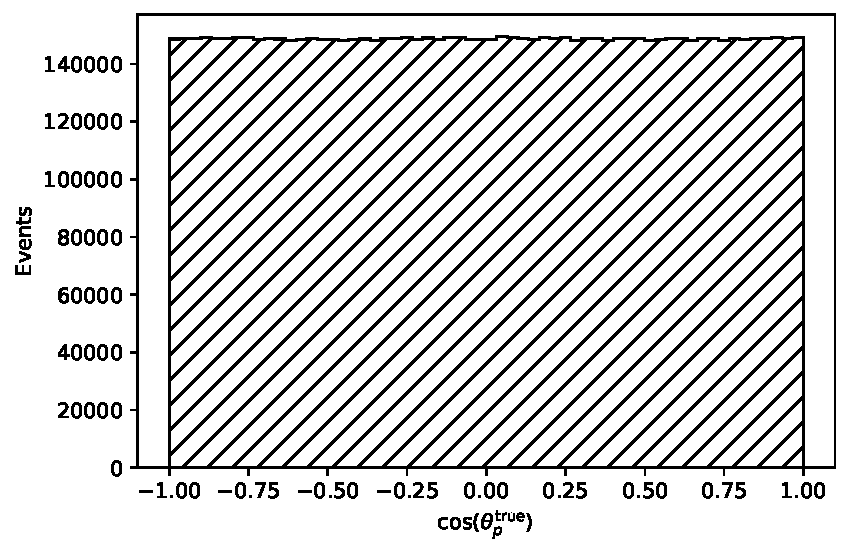
\includegraphics[height=.2\textheight]{graphics/05-angular_distributions/MCTRUTH_theta_true.pdf}
		\caption{}
		\label{fig:5:MCTRUTH_theta_true}
	\end{subfigure}
	\begin{subfigure}{.45\textwidth}
		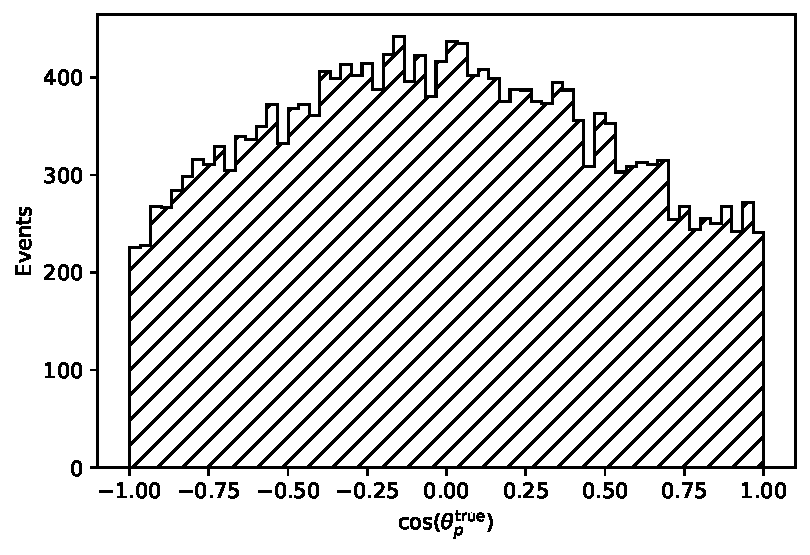
\includegraphics[height=.2\textheight]{graphics/05-angular_distributions/MCRECO_theta_true.pdf}
		\caption{}
		\label{fig:5:MCRECO_theta_true}
	\end{subfigure}
	\vskip .5\baselineskip
	\begin{subfigure}{.45\textwidth}
		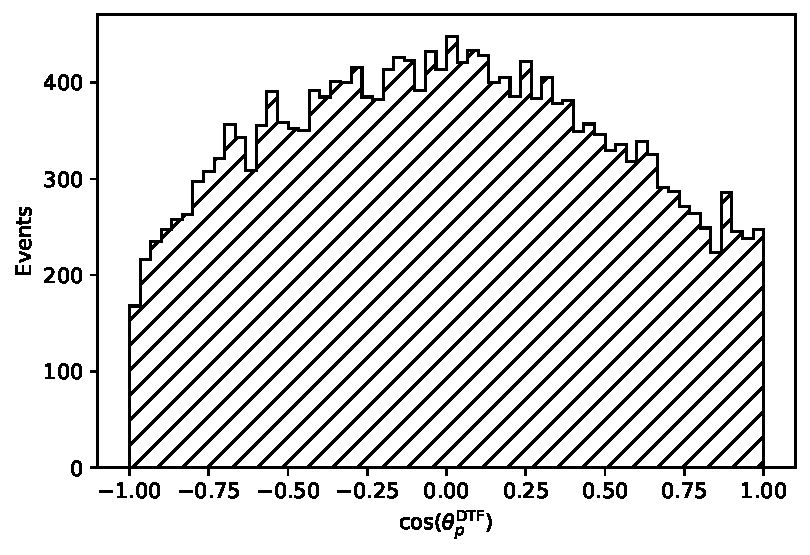
\includegraphics[height=.2\textheight]{graphics/05-angular_distributions/MCRECO_theta_reco.pdf}
		\caption{}
		\label{fig:5:MCRECO_theta_reco}
	\end{subfigure}
	\caption{A.}
	\label{fig:5:theta_distributions}
\end{figure}

\begin{figure}[t]
	\centering
	\begin{subfigure}{.45\textwidth}
		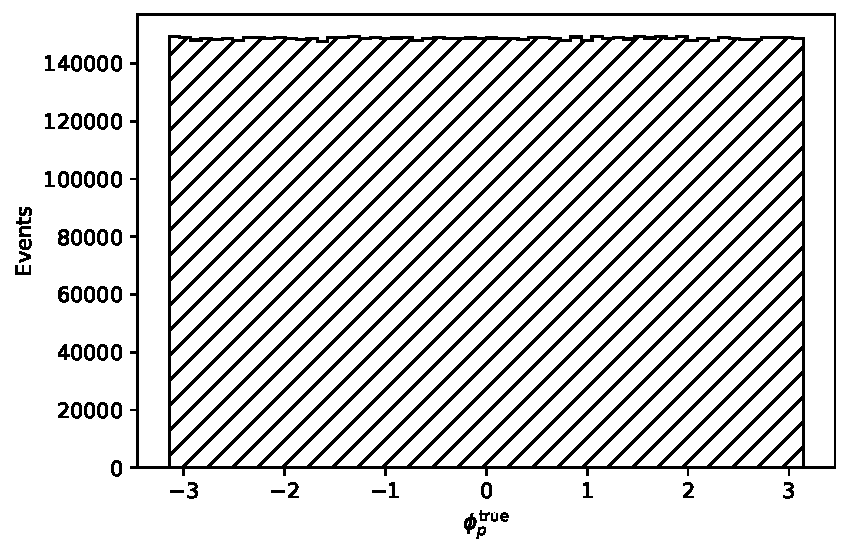
\includegraphics[height=.2\textheight]{graphics/05-angular_distributions/MCTRUTH_phi_true.pdf}
		\caption{}
		\label{fig:5:MCTRUTH_phi_true}
	\end{subfigure}
	\begin{subfigure}{.45\textwidth}
		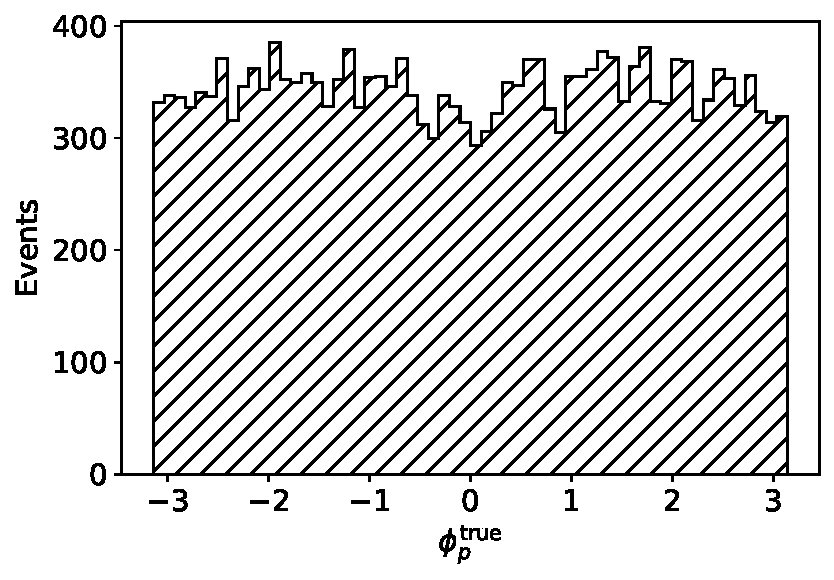
\includegraphics[height=.2\textheight]{graphics/05-angular_distributions/MCRECO_phi_true.pdf}
		\caption{}
		\label{fig:5:MCRECO_phi_true}
	\end{subfigure}
	\vskip .5\baselineskip
	\begin{subfigure}{.45\textwidth}
		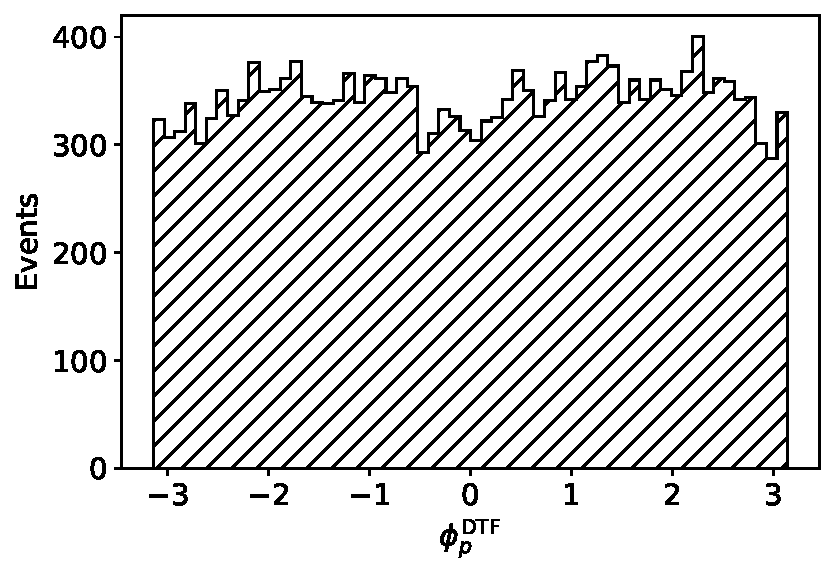
\includegraphics[height=.2\textheight]{graphics/05-angular_distributions/MCRECO_phi_reco.pdf}
		\caption{}
		\label{fig:5:MCRECO_phi_reco}
	\end{subfigure}
	\caption{A.}
	\label{fig:5:phi_distributions}
\end{figure}

\section{Angular distribution resolution}

\begin{figure}[t]
	\centering
	\begin{subfigure}{.45\textwidth}
		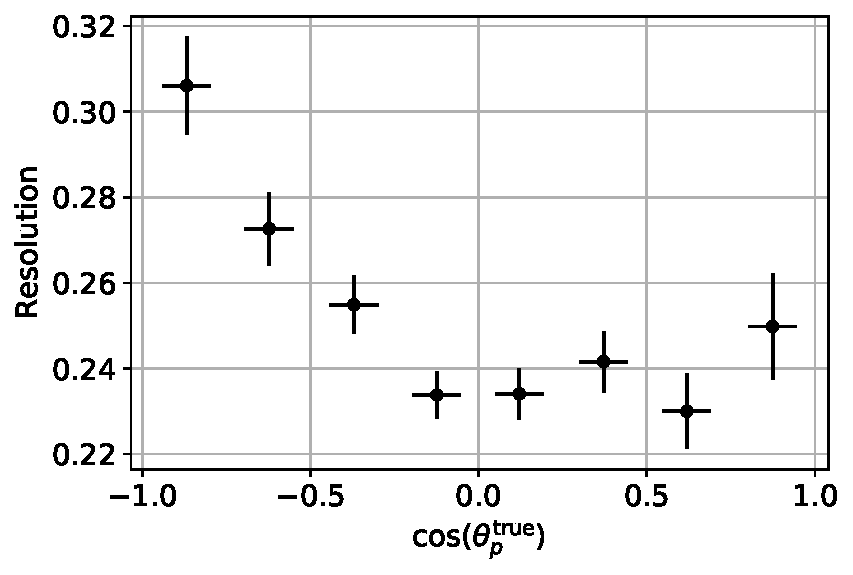
\includegraphics[height=.2\textheight]{graphics/05-angular_distributions/MCRECO_p_theta_resolution.pdf}
		\caption{}
		\label{fig:5:MCRECO_p_theta_resolution}
	\end{subfigure}
	\begin{subfigure}{.45\textwidth}
		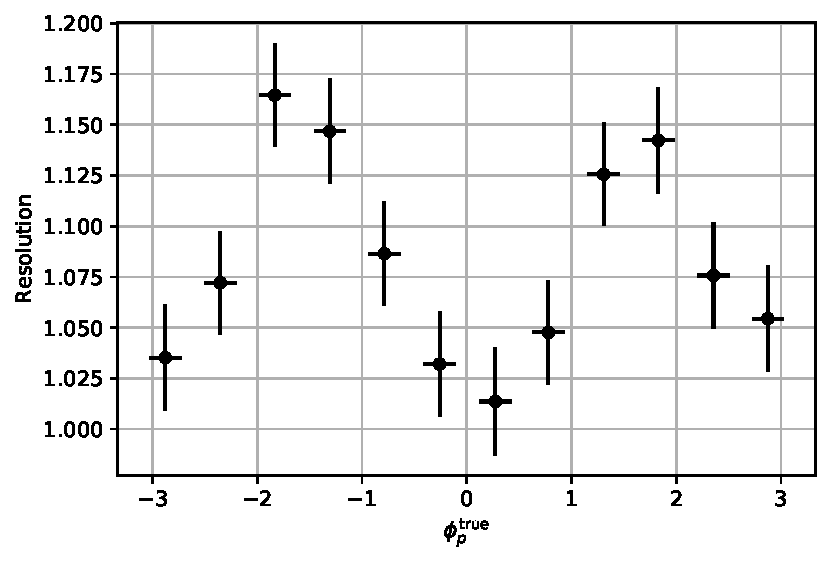
\includegraphics[height=.2\textheight]{graphics/05-angular_distributions/MCRECO_p_phi_resolution.pdf}
		\caption{}
		\label{fig:5:MCRECO_p_phi_resolution}
	\end{subfigure}
	\caption{A.}
	\label{fig:5:angular_resolutions}
\end{figure}

\begin{figure}[t]
	\centering
	\begin{subfigure}{.45\textwidth}
		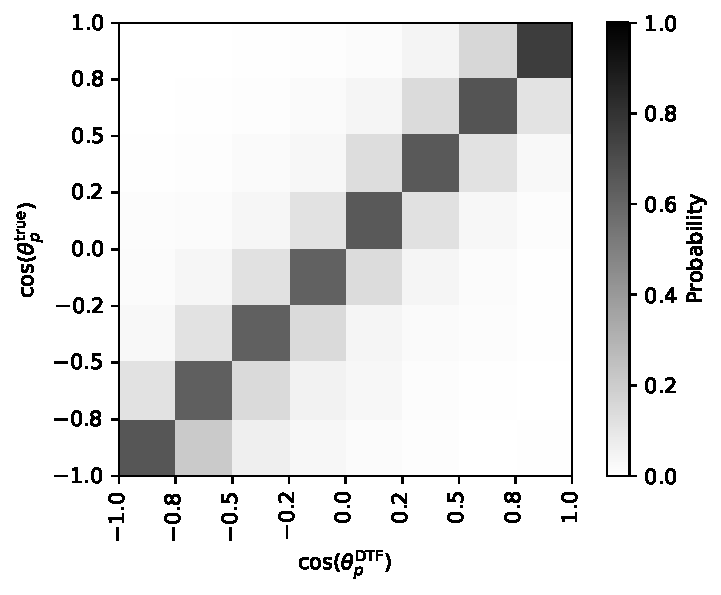
\includegraphics[width=\textwidth]{graphics/05-angular_distributions/MCRECO_p_theta_migration.pdf}
		\caption{}
		\label{fig:5:MCRECO_p_theta_migration}
	\end{subfigure}
	\begin{subfigure}{.45\textwidth}
		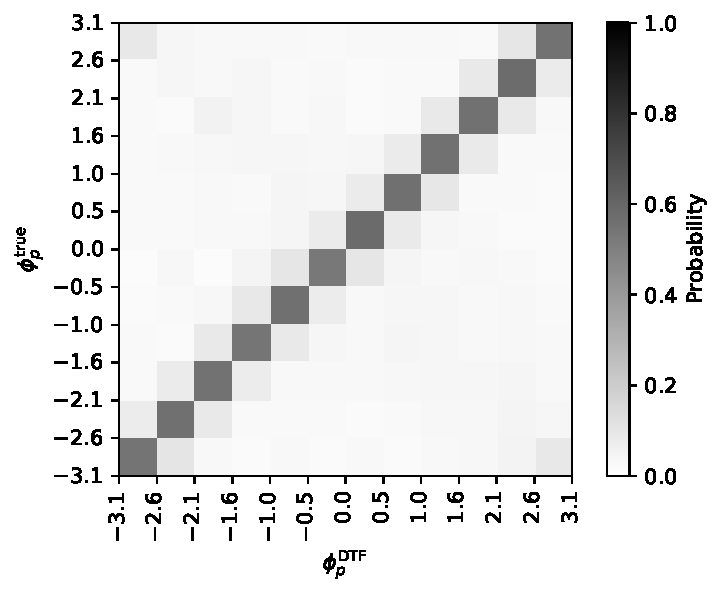
\includegraphics[width=\textwidth]{graphics/05-angular_distributions/MCRECO_p_phi_migration.pdf}
		\caption{}
		\label{fig:5:MCRECO_p_phi_migration}
	\end{subfigure}
	\caption{A.}
	\label{fig:5:angular_migration_matrices}
\end{figure}

\begin{figure}[t]
	\centering
	\begin{subfigure}{.45\textwidth}
		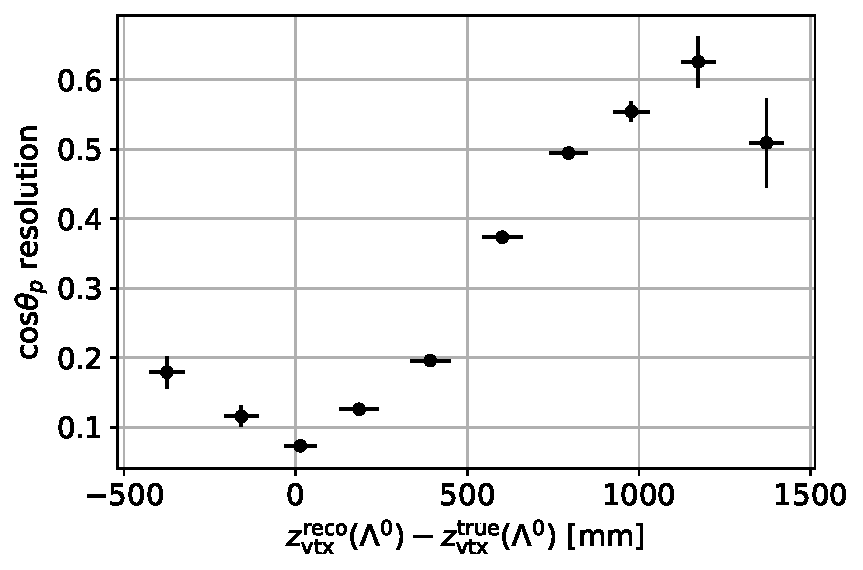
\includegraphics[width=\textwidth]{graphics/05-angular_distributions/MCRECO_p_theta_resolution_vs_L_endvertex_z_bias.pdf}
		\caption{}
		\label{fig:5:theta_resolution_vs_vertex_bias}
	\end{subfigure}
	\begin{subfigure}{.45\textwidth}
		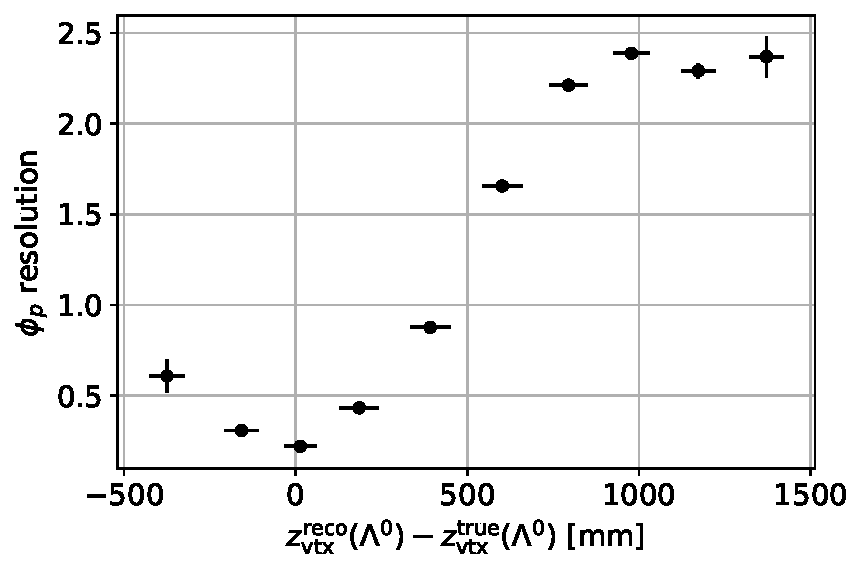
\includegraphics[width=\textwidth]{graphics/05-angular_distributions/MCRECO_p_phi_resolution_vs_L_endvertex_z_bias.pdf}
		\caption{}
		\label{fig:5:phi_resolution_vs_vertex_bias}
	\end{subfigure}
	\caption{A.}
	\label{fig:5:angular_resolution_vs_vertex_bias}
\end{figure}

\subsection{\texorpdfstring{\lz}{Lambda} decay vertex bias and double-crossing tracks}
\label{sec:lambda_endvertex_bias}

The quality of the \lambdadecay vertex reconstruction affects many aspects of the $\Lambda^0$ electromagnetic dipole moments measurement:
on top of being fundamental to evaluate how much magnetic field the particle traversed (and thus the extent of spin precession), even the best momentum resolution for protons and pions is worthless if the particles are extrapolated at the wrong point of production.
Both $x_\text{vtx}^\Lambda$ and $y_\text{vtx}^\Lambda$ are fairly well reconstructed in prefiltered events, with resolution $\lesssim \SI{1}{\centi\meter}$ and no discernible bias.
This section will therefore focus on the reconstruction of $z_\text{vtx}^\Lambda$.

\begin{figure}[t]
	\centering
	\begin{subfigure}{.45\textwidth}
		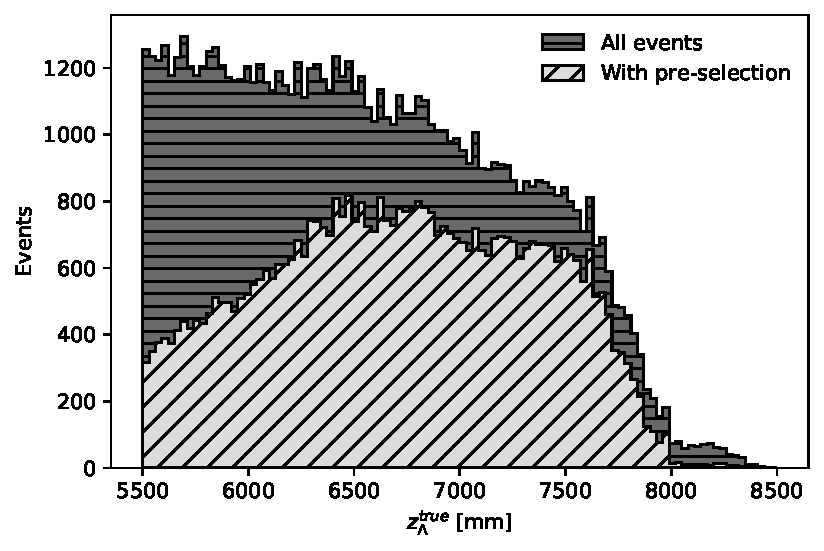
\includegraphics[height=.2\textheight]{graphics/04-event_selection/Lambda_endvertex_z_true.pdf}
		\caption{}
		\label{fig:4:lz_vertex_true}
	\end{subfigure}
	\begin{subfigure}{.45\textwidth}
		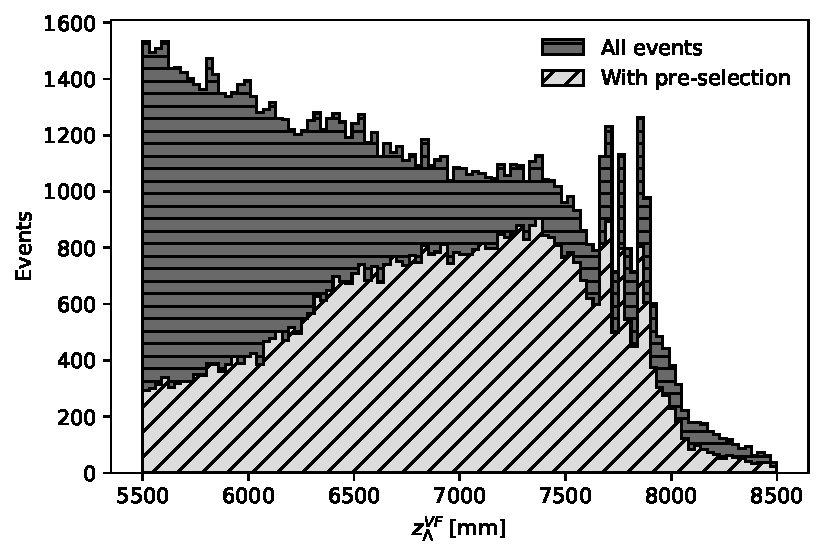
\includegraphics[height=.2\textheight]{graphics/04-event_selection/Lambda_endvertex_z.pdf}
		\caption{}
		\label{fig:4:lz_vertex_reco}
	\end{subfigure}
	\caption{Distribution of true \textit{(a)} and reconstructed \textit{(b)} $z_\text{vtx}^\Lambda$ in simulated \demonstratorshort signal events, without (\textit{dark grey}) and with (\textit{light grey}) prefiltering.}
	\label{fig:4:lz_vertex_distributions}
\end{figure}

\begin{figure}[t]
	\centering
	\begin{subfigure}{.45\textwidth}
		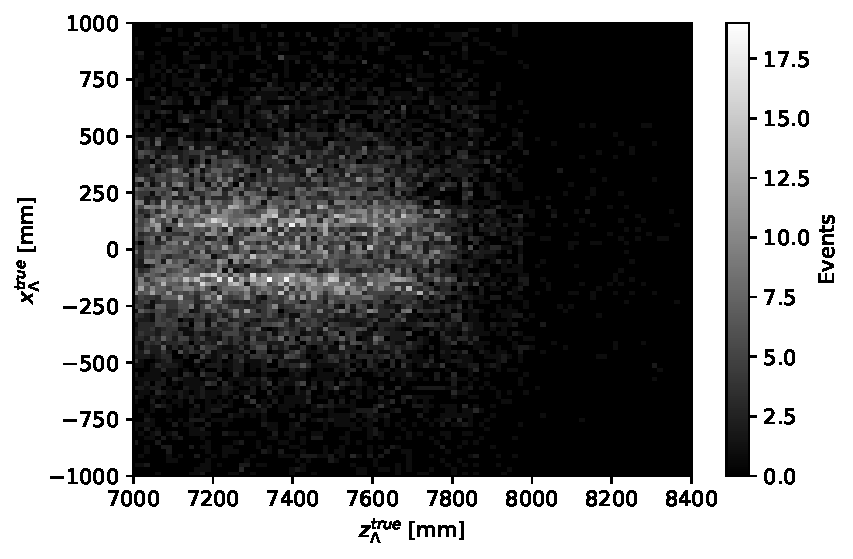
\includegraphics[height=.2\textheight]{graphics/04-event_selection/Lambda_endvertex_z_vs_x_true.pdf}
		\caption{}
		\label{fig:4:lz_vertex_peaks_true}
	\end{subfigure}
	\begin{subfigure}{.45\textwidth}
		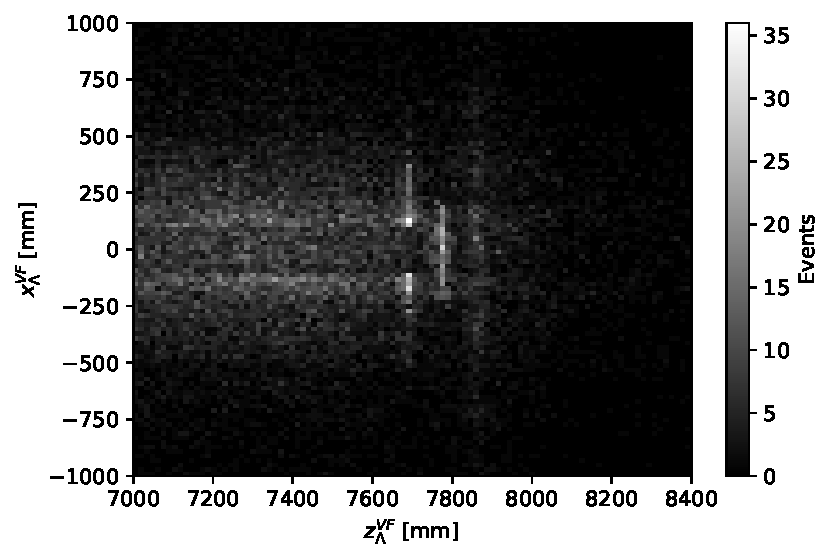
\includegraphics[height=.2\textheight]{graphics/04-event_selection/Lambda_endvertex_z_vs_x.pdf}
		\caption{}
		\label{fig:4:lz_vertex_peaks_reco}
	\end{subfigure}
	\caption{Distribution of simulated \demonstratorshort signal events (prefilters applied) with $z_\Lambda^\text{VF} \geq \SI{7.0}{\meter}$, as function of true (\textit{left}) and reconstructed (\textit{right}) $x_\Lambda^\text{vtx}$ and $z_\text{vtx}^\Lambda$. This corresponds to a top view of true and reconstructed \lz decay vertices.}
	\label{fig:4:lz_vertex_peaks}
\end{figure}

Figures \ref{fig:4:lz_vertex_true} and \ref{fig:4:lz_vertex_reco} show the distributions of true and reconstructed $z_\text{vtx}^\Lambda$ respectively for simulated signal events.
The most prominent difference between the two is the presence of three peaks in the $[\SI{7.5}{\meter},\SI{8.0}{\meter}]$ region of the reconstructed distribution, being found both with and without prefilter selections. 
The significance of these structures can be inferred by plotting the events as function of  $z_\text{vtx}^\Lambda$ and $x_\text{vtx}^\Lambda$, corresponding to a bending plane perspective of the detector.
This is shown in Figure \ref{fig:4:lz_vertex_peaks_reco}, highlighting the fact that the peaks in $\Lambda^0$ decay vertices have a very precise geometrical location, absent when comparing the true $z_\text{vtx}^\Lambda$ and $x_\text{vtx}^\Lambda$ values for the same events (Figure \ref{fig:4:lz_vertex_peaks_true}).
The spatial distribution of the vertices bears a striking resemblance to the layout of a T tracking station (see Figure \ref{fig:2:t_station_top}) and $z$ coordinates are consistent with the nominal placement of IT and first OT plane of the T1 station \cite{Barbosa-Marinho:582793}.
While dedicated studies are required to gain more insight into the source of these structures, they are assumed to be of minor impact for the purposes of this thesis.

\begin{figure}[t]
	\centering
	\begin{subfigure}{.45\textwidth}
		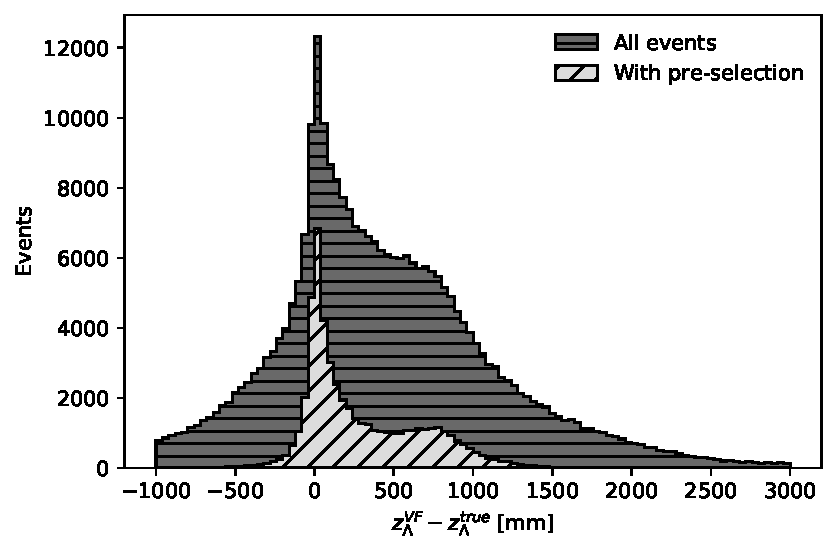
\includegraphics[width=\textwidth]{graphics/04-event_selection/Lambda_endvertex_bias_z.pdf}
		\caption{}
		\label{fig:4:lz_endvertex_bias_linear}
	\end{subfigure}
	\begin{subfigure}{.45\textwidth}
		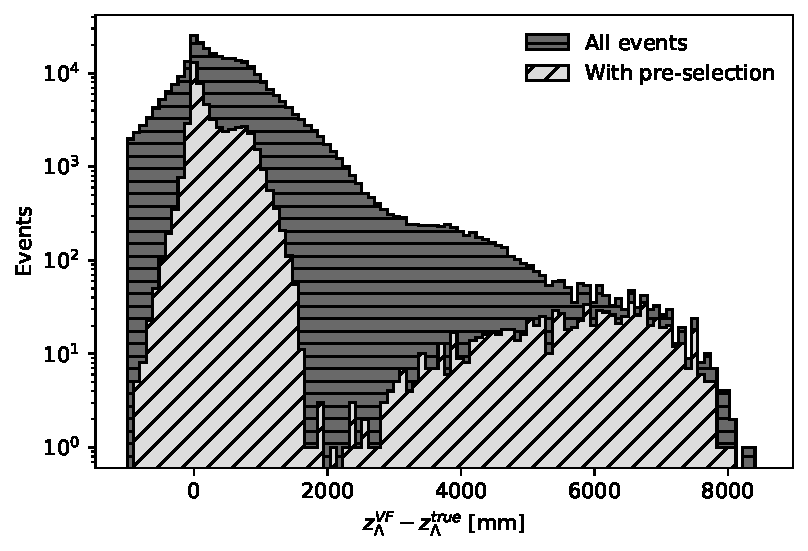
\includegraphics[width=\textwidth]{graphics/04-event_selection/Lambda_endvertex_bias_z_log.pdf}
		\caption{}
		\label{fig:4:lz_endvertex_bias_log}
	\end{subfigure}
	\caption{Distribution of $z_\text{vtx}^\Lambda$ bias for simulated \demonstratorshort events in linear \textit{(a)} and logarithmic \textit{(b)} scales, without (\textit{dark grey}) and with (\textit{light grey}) prefiltering.}
	\label{fig:4:lz_endvertex_bias}
\end{figure}

The differing shapes of true and reconstructed $z_\text{vtx}^\Lambda$ distributions from Figure \ref{fig:4:lz_vertex_distributions} are also evidence of bias effects in the \lambdadecay vertex reconstruction.
This is confirmed in Figure \ref{fig:4:lz_endvertex_bias_linear}, showing the distribution of $z_\text{vtx}^\Lambda$ bias for simulated signal events:
the shape is distinctly non-gaussian, with a long tail towards the positive end of the axis counterbalancing the expected $\approx 0$ peak.
The resulting median bias is $\approx \SI{44}{\centi\meter}$.

\begin{figure}[t]
	\centering
	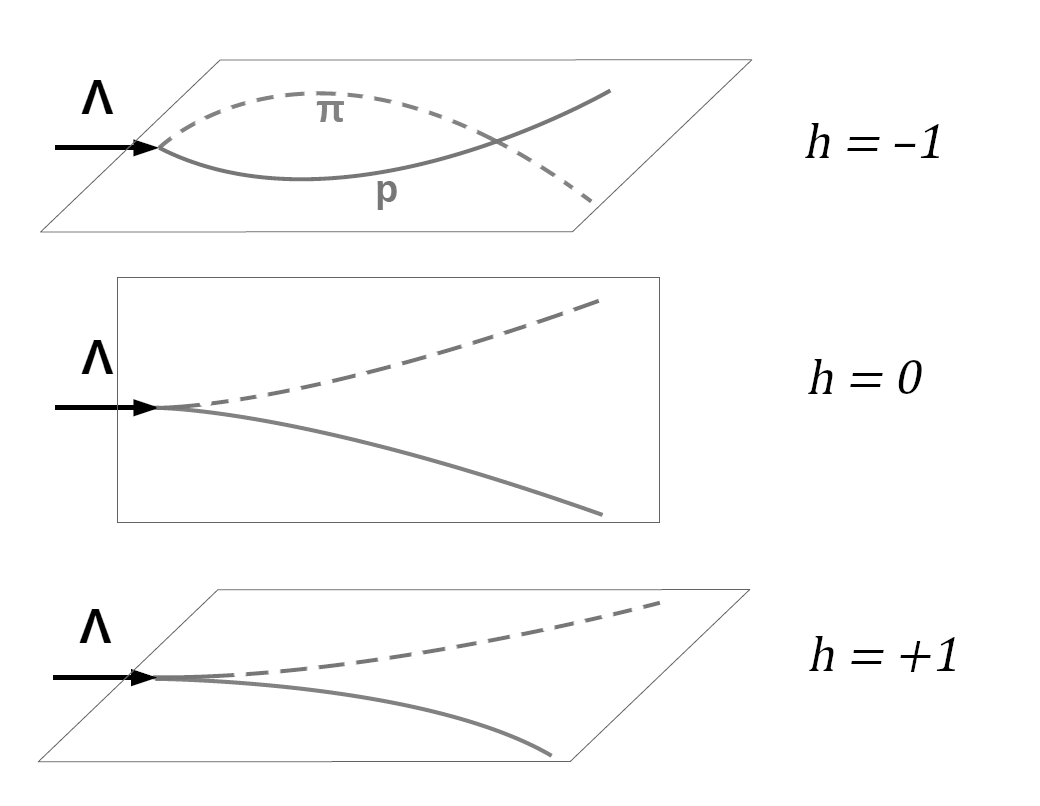
\includegraphics[width=.7\textwidth]{graphics/04-event_selection/horizontality_illustration_bw.png}
	\caption{Depiction of three \lambdadecay configurations and the associated horizontality values. The horizontal planes in the top and bottom diagrams are aligned to the LHCb $xz$ plane, the vertical plane in the middle diagram to the $yz$ plane.}
	\label{fig:4:horizontality_explanation}
\end{figure}

The positive bias tail can be interpreted as a mistake the vertexing algorithm commits when confronted with a specific decay geometry.
When the \lambdadecay decay plane closely aligns with the $xz$ bending plane, the bending induced by the magnet can produce either \textit{opening} or \textit{closing} tracks (depicted in top and bottom diagrams respectively in Figure \ref{fig:4:horizontality_explanation}.
In the latter case the tracks will cross again at $z>z_\text{vtx}^\Lambda$;
if $y$ displacement is sufficiently small, the algorithms converges on this <<ghost>> vertex instead of the real one.

\begin{figure}[t]
	\centering
	\begin{subfigure}{.45\textwidth}
		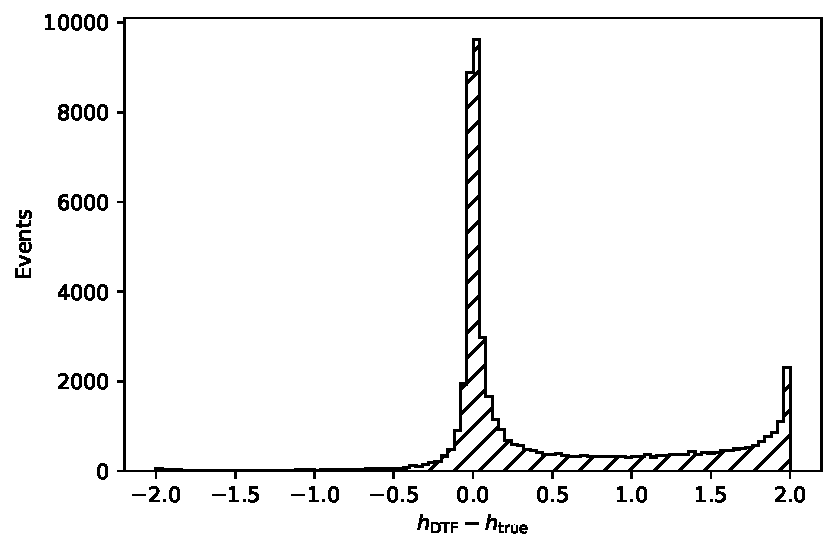
\includegraphics[width=\textwidth]{graphics/04-event_selection/Lambda_horizontality_bias.pdf}
		\caption{}
		\label{fig:4:horizontality_bias}
	\end{subfigure}
	\begin{subfigure}{.45\textwidth}
		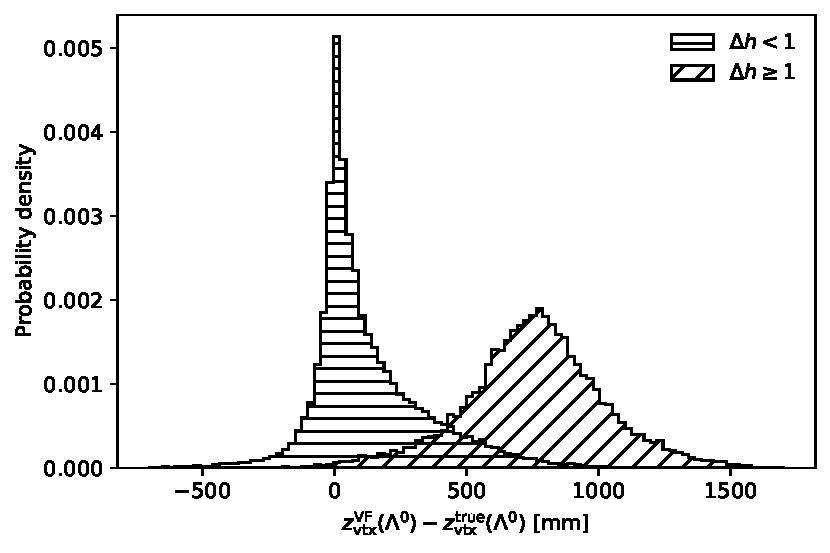
\includegraphics[width=\textwidth]{graphics/04-event_selection/lambda_endvertex_z_bias_vs_horizontality_bias.pdf}
		\caption{}
		\label{fig:4:lz_endvertex_bias_vs_horizontality_bias}
	\end{subfigure}
	\caption{\textit{(a)} Horizontality bias distribution for simulated \demonstratorshort events (prefilters applied), comparing results from Decay Tree Fitter algorithm with \jpsi and \lz mass constraints with true values. \textit{(b)} Distribution of $z_\text{vtx}^\Lambda$ bias for events with horizontality bias $<1$ (\textit{horizontal hatching}) and $\geq 1$ (\textit{diagonal hatching}).}
\end{figure}

To test out this hypothesis we define the \textit{horizontality} of a \lambdadecay event as follows:
\begin{equation}
h = \sign{\left(\Lambda^0_\text{PID}\right)} \sign{\left(B_y\right)}~\frac{a_y}{\lvert \vec{a} \rvert},
\label{eq:4:horizontality}
\end{equation}
where
\begin{equation}
\vec{a} \coloneqq \vec{p}_p \times \vec{p}_\pi 
\end{equation}
is the cross product of proton and pion momenta at production vertex, $\sign{\left(B_y\right)}$ is the dipole magnet polarity\footnote{The LHCb dipole magnet polarity is reversed roughly twice per month to allow for studies on decay asymmetries \cite{Vesterinen:1642153}. The $B_y > 0$ configuration is conventionally known as \textit{magnet up} polarity, $B_y < 0$ as \textit{magnet down}.}
and $\sign{\left(\Lambda^0_\text{PID}\right)}$ is the sign of the PDG Monte Carlo particle numbering scheme of the mother particle ($+1$ for $\Lambda^0$, $-1$ for $\bar{\Lambda}^0$) \cite{PDG}.

Decays with $h=\pm1$ lie exactly on the $xz$ bending plane, $h=-1$ events having closing $p\pi^-$/$\bar{p}\pi^+$ tracks and $h=+1$ events having opening tracks, while $h=0$ events lie on the $yz$ plane (see Figure \ref{fig:4:horizontality_explanation}).
A horizontality bias $\Delta h \coloneqq h_\text{reco} - h_\text{true} > 1$ thus becomes the signature of a <<ghost>> vertex \lambdadecay event.
As per Figure \ref{fig:4:horizontality_bias}, this issue affects $\approx 25\%$ of reconstructed \demonstratorshort events, most of those being $\Delta h \approx 2$ events (from $h=-1$ to $h=+1$), with almost no event with $\Delta h < -1$.

Isolating $\Delta h \geq 1$ events and studying their $z_\text{vtx}^\Lambda$ bias distributions (Figure \ref{fig:4:lz_endvertex_bias_vs_horizontality_bias}), it becomes clear that they are largely responsible for the high bias observed in Figure \ref{fig:4:lz_endvertex_bias_linear}.
Significant asymmetry effects are still visible in the $\Delta h < 1$ distribution, which is still skewed towards positive bias.
While not ideal, this is somewhat expected given that the Vertex Fitter algorithm scans for candidate vertices starting from the first measurement position (i.e. the T1--T3 stations) and moving upstream.

\begin{figure}[t]
	\centering
	\begin{subfigure}{.45\textwidth}
		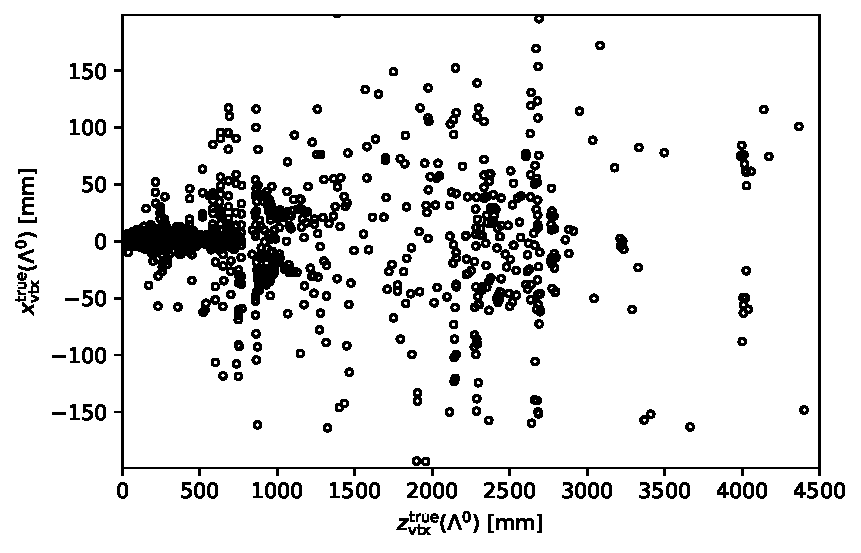
\includegraphics[width=\textwidth]{graphics/04-event_selection/bump_Lambda_true_endvertex_z_vs_x.pdf}
		\caption{}
		\label{fig:4:bump_true}
	\end{subfigure}
	\begin{subfigure}{.45\textwidth}
		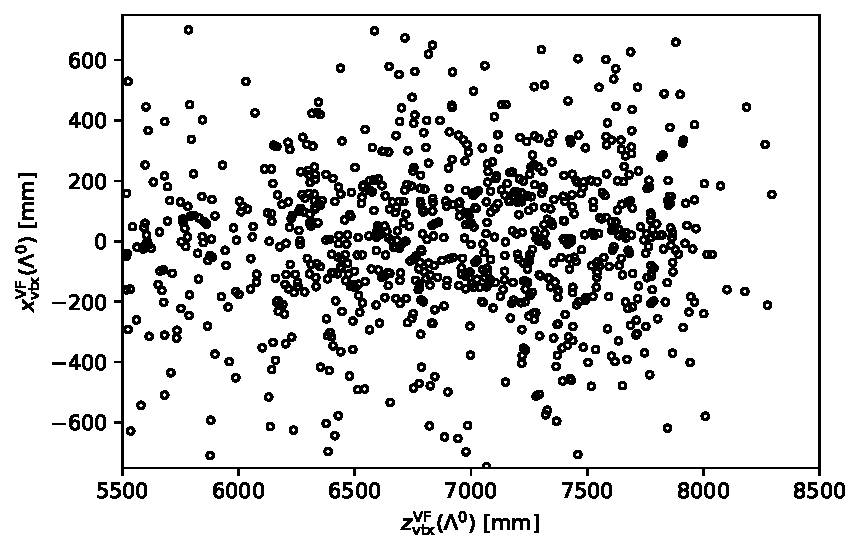
\includegraphics[width=\textwidth]{graphics/04-event_selection/bump_scatter_Lambda_endvertex_z_vs_x.pdf}
		\caption{}
		\label{fig:4:bump_reco}
	\end{subfigure}
	\caption{Distribution of simulated \demonstratorshort events (prefilters applied) with $z_\Lambda^\text{VF} - z_\Lambda^\text{true} \geq \SI{2.0}{\meter}$ as function of true \textit{(a)} and reconstructed \textit{(b)} $x_\Lambda^\text{vtx}$ and $z_\text{vtx}^\Lambda$. This corresponds to a top view of true and reconstructed \lz decay vertices.}
	\label{fig:4:bump}
\end{figure}

Most \demonstratorshort events, even those with ghost vertex reconstruction, still maintain a limited $\lesssim \SI{1.0}{\meter}$ bias on $z_\text{vtx}^\Lambda$.
A smaller substructure with $\geq \SI{2.0}{\meter}$ bias emerges when plotting the distribution in logarithmic scale, as in Figure \ref{fig:4:lz_endvertex_bias_log}.
Figure \ref{fig:4:bump_true} provides a top view of the $\Lambda^0$ decay vertices of these evemts, showing the distribution of true $z_\text{vtx}^\Lambda$ and $x_\text{vtx}^\Lambda$.
Most $\Lambda^0$ in high bias events decay in the earlier sections of the detector ($z<\SI{3.0}{\meter}$);
the high spatial concentration in specific regions of the $xz$ plane, such as the <<wings>> around $z\approx \SI{1.0}{\meter}$, as well as the consistency between the placement of these structures and the location of the different LHCb subdetectors (cf. Figure \ref{fig:2:lhcb_diagram}), suggest that they may be the result of interaction with the material.

No selection on reconstructed variables is possible to filter this class of events:
Figure \ref{fig:4:bump_reco} shows that the $\Lambda^0$ vertices are reconstructed in seemingly arbitrary positions.
Their impact on the overall performance on signal is nevertheless neglectable, since this events amount to roughly 1.7\% of the prefiltered simulated sample.

\subsection{Impact of double-crossing decays on angular resolution}